\documentclass{beamer}

\usetheme{Madrid}
\usecolortheme{whale}
\usepackage{xcolor}
\usepackage{etoolbox}

\usepackage{graphicx}
\usepackage{hyperref}
\usepackage[backend=biber, sorting=none]{biblatex}
\addbibresource{refs.bib}
\DeclareFieldFormat*{title}{#1}
\DeclareFieldFormat*{url}{\newline\url{#1}\nopunct}
\DeclareFieldFormat{labelnumberwidth}{#1\adddot}
\setlength{\biblabelsep}{5pt}
\renewcommand*{\bibfont}{\tiny}
\usepackage{ragged2e}

\newcommand{\biburl}[2][]{%
  \newline - \ifstrempty{#1}{}{\textcolor{cyan}{#1: }}\url{#2}\nopunct
}

\newcounter{lesson_cnt}
\newcommand{\lesson}[1]{
  \stepcounter{lesson_cnt}
  \section{Lesson \arabic{lesson_cnt}: #1}
  \subtitle{Lesson \arabic{lesson_cnt}: #1}
  \begin{frame}
    \titlepage
  \end{frame}
  
  \begin{frame}{Outline of Lesson \arabic{lesson_cnt}}
    % \tableofcontents[currentsection,hideothersubsections]
    \tableofcontents[sections={\arabic{lesson_cnt}}]
  \end{frame}
}

\title{GPT Survey: A Programmer's Perspective}
\author{Yu Zehan}
\institute{Intel FLEX}
\date{\today}

\begin{document}

\begin{frame}
  \titlepage
\end{frame}

\begin{frame}{Outline}
  \tableofcontents[hideallsubsections]
\end{frame}

% Lesson 1
\lesson{Prompt Engineering: Principles, Techniques, and Tools}
% 行动指南(instructions)、事实依据(facts)、思想纲领(policies)

\subsection{Prompt Workflows}

\begin{frame}{Prompt Workflow}
\end{frame}

\subsection{Prompt Principles}
\begin{frame}{Prompt Principles}
% More details and examples
  % One-shot or Few shots
% Structured
  % Delimiters
  % Formatted instructions and examples
% Iterate
  % Step by step
  % self-check
% Top to Bottom
  % Divide and conquer
  

  % More details
  % Do One Thing And Do It Well (DOTADIW)
  % Iteration 
  % Shots
  % Structured Inputs and Outputs
  % Search Engine is still powerful
\end{frame}

\subsection{Prompt Techniques}
\begin{frame}{Prompt Techniques}
  % Use delimiters
  % Ask for structured output
  % Instruct the model to check conditions
  % Use few-shot prompting.
  
  % Workflow: Role -> Instruction -> Examples -> Context -> Question
  % autogpt: Task -> Reason -> Plan -> Criticize -> Act -> Iterate
\end{frame}

\begin{frame}{Think Like LLM}
  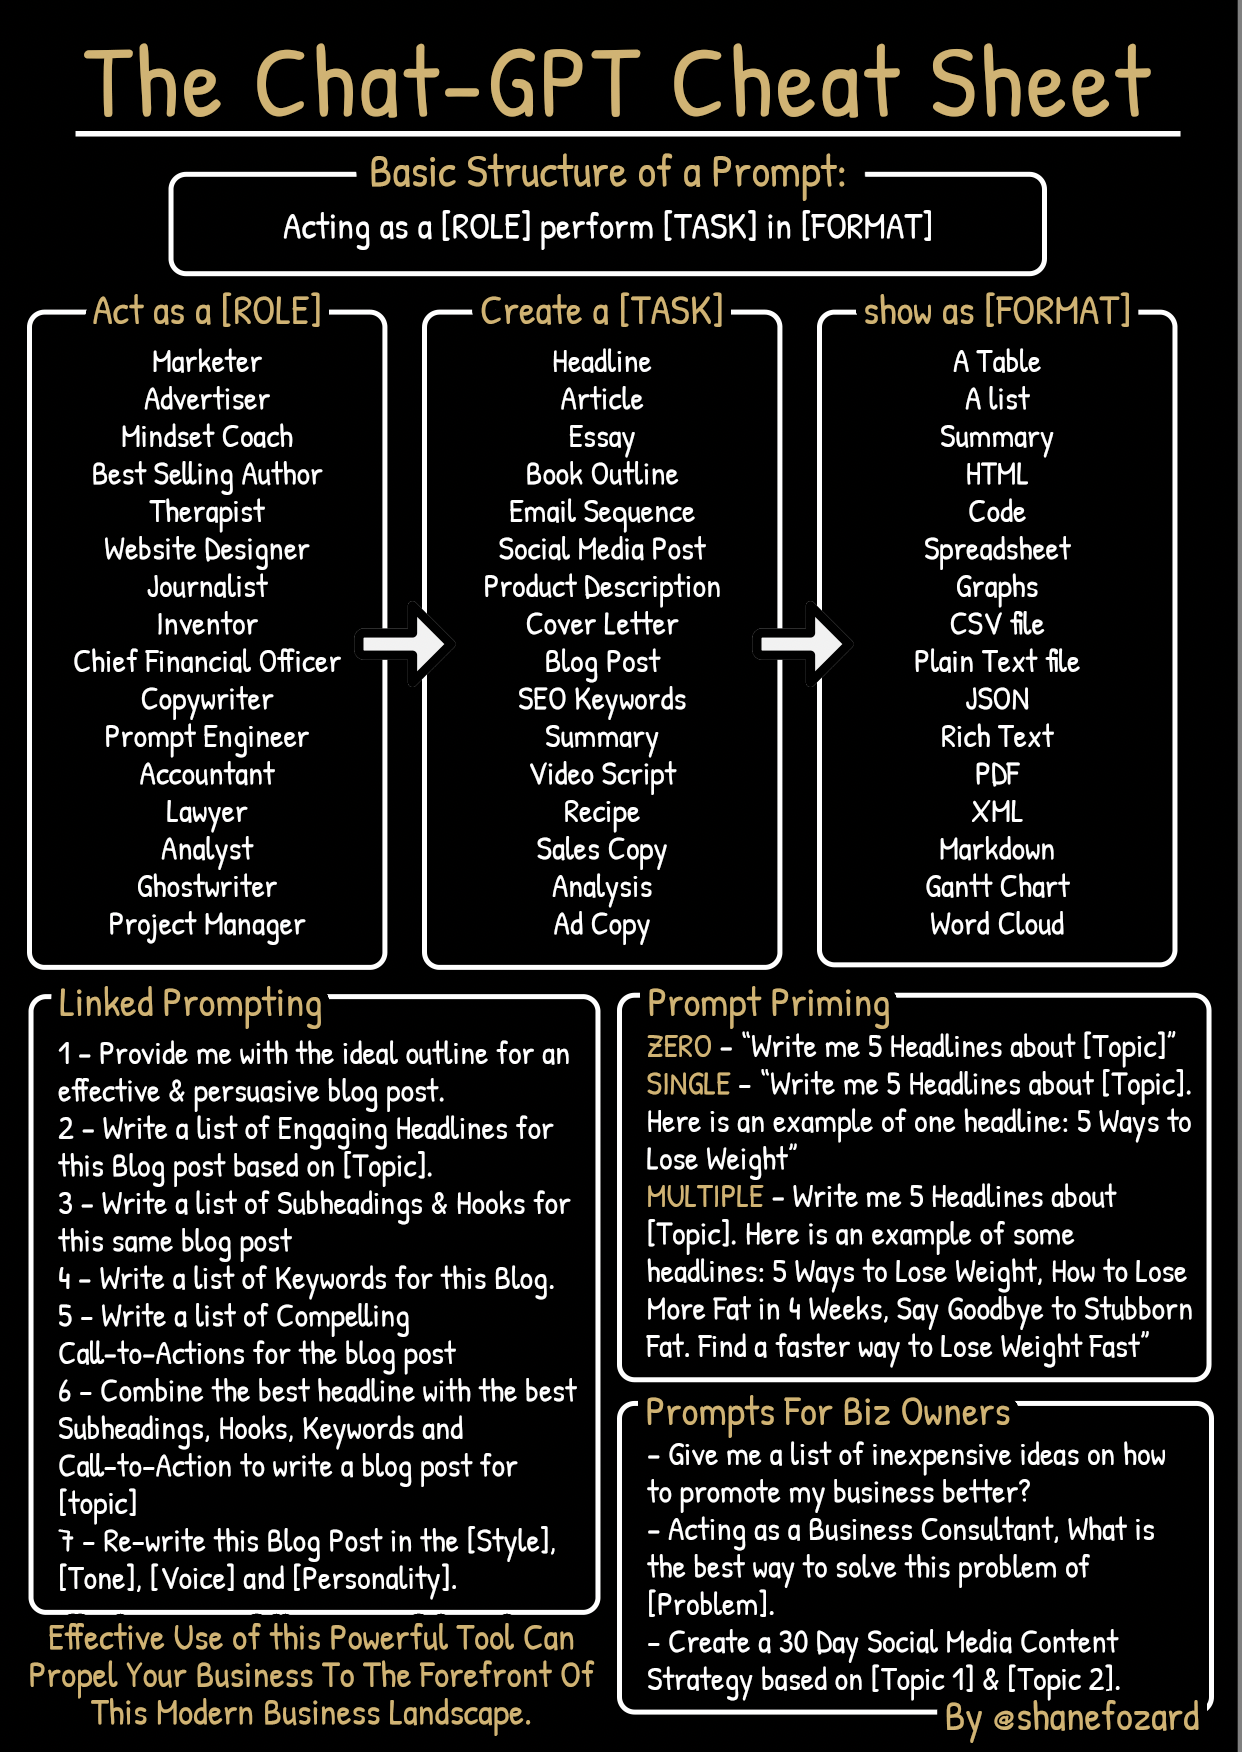
\includegraphics[width=\textwidth,height=0.8\textheight,keepaspectratio]{./images/chatgpt-cheatsheet.png}
\end{frame}

\subsection{Tools and Extensions}
\begin{frame}{Tools and Extensionsle}
  
\end{frame}

% Lesson 2
\lesson{Case Studies of Coding Tasks with GPT}
\begin{frame}
  \titlepage
\end{frame}

% Lesson 3
\lesson{Integrate GPT in Whole Coding Lifecycle}
\begin{frame}
\titlepage
\end{frame}

% Lesson 4
\lesson{Cutting-Edge GPT Projects and Showcases}
\begin{frame}
  \titlepage
\end{frame}

% Lesson 5
\lesson{Customize GPT for More Power}
\begin{frame}
\titlepage
\end{frame}

\begin{frame}
\end{frame}


\section{References}
\begin{frame}[t,allowframebreaks]{References}
  \nocite{*}
  \RaggedRight
  \printbibliography
\end{frame}


\begin{frame}{FAQ}

\end{frame}

\end{document}
